\chapter{Implicitación de superficies}

\section{Introducción}

Las superficies implícitas se usan en la ciencia de computación gráfica desde los años 70 para modelar objetos geométricos, pero su uso e importancia han ido creciendo en años recientes ya que puede ser usados para describir objetos en espacios de dimensión arbitraria. En este Trabajo Fin de Máster nos centraremos en objetos de dimensión dos y tres. Cualquier objeto matemático se puede definir de una forma particular, luego nos cabe preguntarnos porqué las superficies en forma implícita se han popularizado tanto y la respuesta la encontramos en que la expresión implícita de una superficie suele ser compacta y manejable frente a la expresión paramétrica, por ejemplo, la expresión paramétrica de la esfera unidad es la siguiente:

$$X(u,v) = (cos(u)sen(v),sen(u)sen(v),cos(v)) \hspace{1.5cm} (u,v) \in [0,2\pi] \times [0,\pi]$$

Y la forma implícita es:

$$f(x,y,z) = x^2 + y^2 + z^2 - 1$$

Queda claro que en este ejemplo las propiedades que hemos mencionado.
\par 
Aunque hemos mencionado las ventajas de usar la forma implícita para la modelización y visualización de superficies, su principal debilidad es la cantidad de tiempo que necesitan para la visualización directa, véase usando ray tracing. \cite{Groot05} Otra de las debilidades de las superficies en forma implícita es la dificultad de controlar la forma delas superficies durante una visualización rápida en un entorno interactivo.
\par Esto lleva a que las representaciones paramétricas sigan siendo populares hoy en día gracias a la relativamente rápida renderización que presentan.
\par Aún presentando estas debilidades, las superficies son una forma flexible de crear objetos complejos ya que ofrecen una clasificación manejable y clara de conjuntos de puntos, es decir, es fácil saber si un punto del espacio se encuentra { \em dentro}, { \em fuera} o en la superficie.
\par Además también se pueden usar para la representación de nubes de puntos, por ejemplo, en imágenes de datos médicos y reconstrucción de objetos representados como medias de conjuntos de puntos. \cite{Benedet05} \cite{Peiro06}

\section{Descripción del problema}

Una superficie implícita $S$ se define el conjunto de puntos $p \equiv (x,y,z) \in \mathbb{R}^3$ que verifican la ecuación $f(p) = 0$, donde $f : \mathbb{R}^3 \to \mathbb{R}$ es una función que asigna un valor escalar a cada punto del espacio. Es decir:

$$S = \{ p \in \mathbb{R}^3 : f(p) = 0 \}$$

Sea $A$ el sólido cerrado descrito por por la función implícita $f$, por uniformidad consideraremos el siguiente criterio:

$$\begin{tabular}{l c l}
    $p \in int(A)$ & $\iff$ & $f(p) < 0$ \\
    $p \in \partial A$ & $\iff$ & $f(p) = 0$ \\
    $p \in ext(A)$ & $\iff$ & $f(p) > 0$
\end{tabular}$$

Donde $int(A)$, $\partial A$ y $ext(A)$ denotan el interior, frontera y exterior del sólido cerrado $A$ respectivamente. Esto establece por medio de la vía topológica que la función implícita es negativa dentro del sólido, cero en la superficie, véase frontera, y positiva en el exterior.\cite{Hart01}

Este sistema es un estándar que se suele usar por comodidad y por ser el más común entre la literatura de este tipo de trabajos. Otros ejemplos incluyen a
\cite{Uhlir03} o \cite{Blinn82} donde las funciones implícitas definidas eran positivas en el interior y negativas en el exterior del sólido, o por ejemplo \cite{Ricci73} donde eran siempre positivas y alcanzaban el valor unidad en la superficie, menos uno en el interior y mayor que uno en el exterior.

Está claro que estas definiciones no afectan al problema principal, véase que, volviendo al ejemplo de la esfera, en \cite{Uhlir03} usan lo que llaman la forma inversa que sería la siguiente:

$$f(x,y,z) = - x^2 - y^2 - z^2 + 1$$

Ahora que hemos descrito las ventajas de las superficies dadas de forma implícita queremos ver los métodos para crear la representación implícita de objetos arbitrarios. Existen dos tipos de guías para la creación de la representación implícita de un objeto.

La primera manera usa la expresión paramétrica  de una primitiva o un { \em parche} como entrada. La representación implícita del objeto se genera usando operaciones simbólicas para la expresión paramétrica. Este tipo de métodos se llaman { \em métodos de eliminación de variables}.

La segunda manera comienza comienza con un mallado poligonal o una nube de puntos. El iso-valor, que provee información sobre una posición particular del punto, puede ser calculado directamente de esta representación. Entonces el iso-valor significa si el punto está dentro, fuera o en la superficie.

\section{Métodos de eliminación de variables}

Eliminación es una disciplina matemática para suprimir variables de sistemas de ecuaciones. En \cite{Hoffmann93} se hace una clasificación del método de la resultante, el método de la base de Gröbner y el método de Wu-Ritt. Todos los métodos que vamos a describir tienen una propiedad común y esta es que el resultado del algoritmo es una ecuación la cual puede ser utilizada por métodos de visualización directa.

\subsection{Método de la base de Gröbner}

Este método se basa en encontrar una base de Gröbner par un ideal $I$, donde éste es un un conjunto ordenado de polinomios que cumple con el requisito de existencia de una base de Gröbner. La búsqueda  de una base de Gröbner reducida se basa en la búsqueda de una solución exacta de un sistema de ecuaciones polinomiales. Si el sistema de ecuaciones polinomiales tiene una solución, entonces las variables de del sistema son eliminadas y el conjunto original de ecuaciones se transforma. Este nuevo conjunto de ecuaciones transformadas sí puede ser solucionado de forma sencilla.

La transformación de la expresión paramétrica en un expresión implícita puede ser resuelto de una forma satisfactoria usando una base de Gröbner de un ideal. Hay dos maneras de resolver la transformación según si la variedad de entrada en polinomial o racional.

\subsubsection*{Ideal}

Sea $I \subset k[x_1, \dotso, x_n]$ se llama ideal en $k[x_1, \dotso, x_n]$ si se verifican las siguientes dos condiciones:

\begin{enumerate}
    \item Si $f, g \in I$, entonces $f + g \in I$.
    \item Si $f \in I$, entonces $fg \in I$ para todo $g \in k[x_1, \dotso, x_n]$.
\end{enumerate}

Sean $f_1, \dotso, f_s \in k[x_1, \dotso, x_n]$, consideramos un ideal $I$ que los contiene. El conjunto $I =  \left\{ \sum_{i=1}^{s} g_i f_i \ : \ g_i \in k[x_1, \dotso, x_n] \right\}$ es un ideal en $k[x_1, \dotso, x_n]$y además es el menor ideal que contiene a los polinomios $f_1, \dotso, f_s$. El conjunto $\left\{ f_1, \dotso, f_s \right\}$ se llama conjunto generador o base del ideal $I$. 

\subsubsection*{Ordenamiento de los polinomios}

Para la computación de la base de Gröbner el ordenamiento de los términos en un polinomio es esencial. De mayor interés son los órdenes totales, que se denotan por $\prec$ y tienen las siguientes propiedades:

\begin{enumerate}
    \item El orden es compatible con un producto.
    \item Para polinomios finitos no puede existir una sucesión infinita decreciente de términos tal que $t_1 \prec t_2 \prec \dotso$
\end{enumerate}

Los esquemas de ordenación más comunes son los siguientes, aunque existe bastante variedad y se pueden escoger según convenga:
\\
\par
\textit{Orden lexicográfico}
\\ \par
Si partimos de las posibles combinaciones de monomios en dos variables $x_1$ y $x_2$ tales que establecemos que $x_1 \prec x_2$ el orden lexicográfico resultante sería:

$$1 \prec x_1 \prec x_1^2 \prec \dotso \prec x_2 \prec x_1 x_2 \prec x_1^2 x_2 \prec \dotso \prec x_2^2 \prec \dotso$$

\bigskip
\textit{Orden graduado}
\\ \par
Este método primero ordena los términos por su grado y los términos de igual grado se ordenan de manera lexicográfica. Tomando el ejemplo anterior nos quedaría:

$$1 \prec x_1 \prec x_2  \prec x_1^2 \prec x_1 x_2 \prec x_2^2 \prec \dotso$$

\subsubsection*{Reducción polinomial}

Para calcular la base de Gröbner es importante elegir un orden $\prec$, por ello tras haberlo elegido pasamos a definir los siguientes términos:

\begin{definition}
Para cada polinomio $f(x_1, \dotso, x_n)$ se define el monomio líder como el mayor término de $f$ bajo $\prec$ con coeficientes no nulos. Se denota por $LM(f)$.
\end{definition}

\begin{remark}
El coeficiente del monomio líder se llama coeficiente líder y se denota por $LC(f)$.
\end{remark}

\begin{definition}
El término líder de un polinomio $f$ se define como el producto del monomio líder y el coeficiente líder y se denota por $LT(f)$.
\end{definition}

\begin{definition}
La cola de un polinomio $f(x_1, \dotso, x_n)$, denotado por $TT(f)$ se obtiene separando el término líder del resto del polinomio.
\end{definition}

Con las definiciones dadas se puede reescribir un polinomio $f(x_1, \dotso, x_n)$ como:

$$f = LT(f) + TT(f)$$

Bien, ahora podemos proceder a la reducción polinomial propiamente dicha. Dados dos polinomios $f(x_1, \dotso, x_n)$ y $g(x_1, \dotso, x_m)$ se dice que $g$ reduce a un polinomio $h$ respecto de $f$ si, y sólo si, $LT(g)$ se puede eliminar mediante la resta de un múltiplo apropiado de $f$. Esta operación se denota por $g \to_f h$.
\par
Por tanto, la reducción $g \to_f h$ es posible si, y sólo si, existe un escalar $b$ y un monomio $u$ tales que $h = g - buf$ donde $b = \frac{LC(g)}{LC(f)}$ y $u =\frac{LM(g)}{LM(f)}$.
\par
Se dice que un polinomio $g$ se reducerespecto de un conjunto, o base, de polinomios $F = \{ f_1, \dotso, f_n \}$ si $g$ es reducible respecto de uno o má polinomios de $F$. En tal caso la reducción de un polinomio puede conducir a una secuencia de reducciones, lo que es un proceso finito. Se puede probar además que cada polinomio $g_i$ en la secuencia de reducciones y el propio polinomio $g$ es un elemento del ideal $(f_1, \dotso, f_n)$.

\subsubsection*{S-polinomios}

Este proceso que hemos llevado a cabo nos conduce a otro tipo de polinomios, los llamados \textbf{S-polinomios}. Para dos polinomios $f$ y $g$ se define su S-polinomio como:

$$S(f,g) = \frac{x^{\gamma}}{LT(f)} \cdot f - \frac{x^{\gamma}}{LT(g)} \cdot g$$

Donde $x^{\gamma}$ representa el mayor monomio común entre los monomio líderes de $f$ y $g$.

\subsubsection*{Base de Gröbner}

Una base de Gröbner de un conjunto de polinomios es un tipo concreto de base de su ideal que cumple:

\begin{itemize}
    \item Todo polinomio en el ideal se reduce a cero respecto a la base.
    \item Todo polinomio tiene una única forma normal respecto de la base.
\end{itemize}

Después de escoger un orden, el conjunto $G = \{ g_1, \dotso, g_l \}$ del ideal $I$ es una base de Gröbner si:

$$\langle LT(g_1), \dotso, LT(g_l) \rangle = \langle LT(I) \rangle$$

Es decir, el conjunto $G \subset I$ es la base de Gröbner si, y sólo si, el término líder de cualquier elemento de $I$ es divisible entre $LT(g_i)$ para todo $i = 1, \dotso, l$.
\par
En el primer caso, donde la parametrización se expresa como polinomios, se puede expresar como:

\begin{equation}
\begin{tabular}{c c c}
$x_1$ & $=$ & $f_1(t_1, \dotso, t_m)$ \\
$\vdots$ & $\vdots$ & $\vdots$ \\
$x_n$ & $=$ & $f_n(t_1, \dotso, t_m)$
\end{tabular}
\nonumber
\end{equation}

donde $f_1, \dotso, f_n$ son polinomios en $K[t_1, \dotso, t_m]$ con $K$ un cuerpo. Este sistema se puede ver como la proyección $F : K^m \to K^n$ definida por:

$$F(t_1,\dotso, t_m) = (f_1(t_1,\dotso, t_m), \dotso, f_n(t_1,\dotso, t_m))$$

Entonces, la imagen de la proyección es un subconjunto de $K^n$ parametrizado por el sistema previo. Teniendo en cuenta que $F(K^m)$ no es una variedad afín, se obtiene que la solución del problema de conversión de ecuaciones paramétricas a implícitas es equivalente a encontrar la variedad mínima que contiene a $F(K^m)$ i.e. el problema de implicitación consiste en laeliminación de parámetros de la descripción paramétrica. La ecuación final contiene solo las variables $x_1, \dotso, x_n$.
\par
La eliminación de variables se puede realizar calculando la base de Gröbner reducida para un ideal $I = \langle x_1 - f_1, \dotso, x_n - f_n \rangle$. Para enfrentarse a este problema solo es necesario tener en cuenta el orden $\prec$.
\par
El segundo método es la implicitación racional, la cual puede ser expresada como:
\begin{equation}
\begin{tabular}{c c c}
$x_1$ & $=$ & $\frac{f_1(t_1, \dotso, t_m)}{g_1(t_1, \dotso, t_m)}$ \\
$\vdots$ & $\vdots$ & $\vdots$ \\
$x_n$ & $=$ & $\frac{f_n(t_1, \dotso, t_m)}{g_n(t_1, \dotso, t_m)}$
\end{tabular}
\nonumber
\end{equation}

donde $f_1, \dotso, f_n, g_1, \dotso, g_n \in K[t_1, \dotso, t_m]$. La proyección $F : K^m \to K^n$ no se puede definir en todo $K^m$ ya que, obviamente, hay que excluir el conjunto de raíces de los polinomios $g_i$ para todo $i = 1, \dotso, n$. Si denotamos como $W \subset K^m$, entonces:

$$F(t_1, \dotso, t_m) = \left( \frac{f_1(t_1, \dotso, t_m)}{g_1(t_1, \dotso, t_m)}, \dotso, \frac{f_n(t_1, \dotso, t_m)}{g_n(t_1, \dotso, t_m)}  \right)$$

define la proyección $F : K^m / W \to K^n $. El objetivo es encontrar la variedad mínima en $K^n$ que contenga $F(K^m / W)$. En la parametrización definida se eliminan las fracciones multiplicando la iésima coordenada por el polinomio $g_i$. Entonces la ecuación $1 - g_1 \dotso g_n y = 0$, ara polinomios $g_i$ no nulos en la variedad definida, se añade  y se evalua la base de Gröbener reducida. Los elementos de la base de Gröbner que no contienen a las variables $t_1, \dotso, t_n, y$ definen la representación implicita de la variedad afín dada.
\par
Una explicación más exhaustiva se puede encontrar en \cite{Hoffmann93}.
\subsubsection*{Ejemplo}

\begin{figure}[h]
\centering
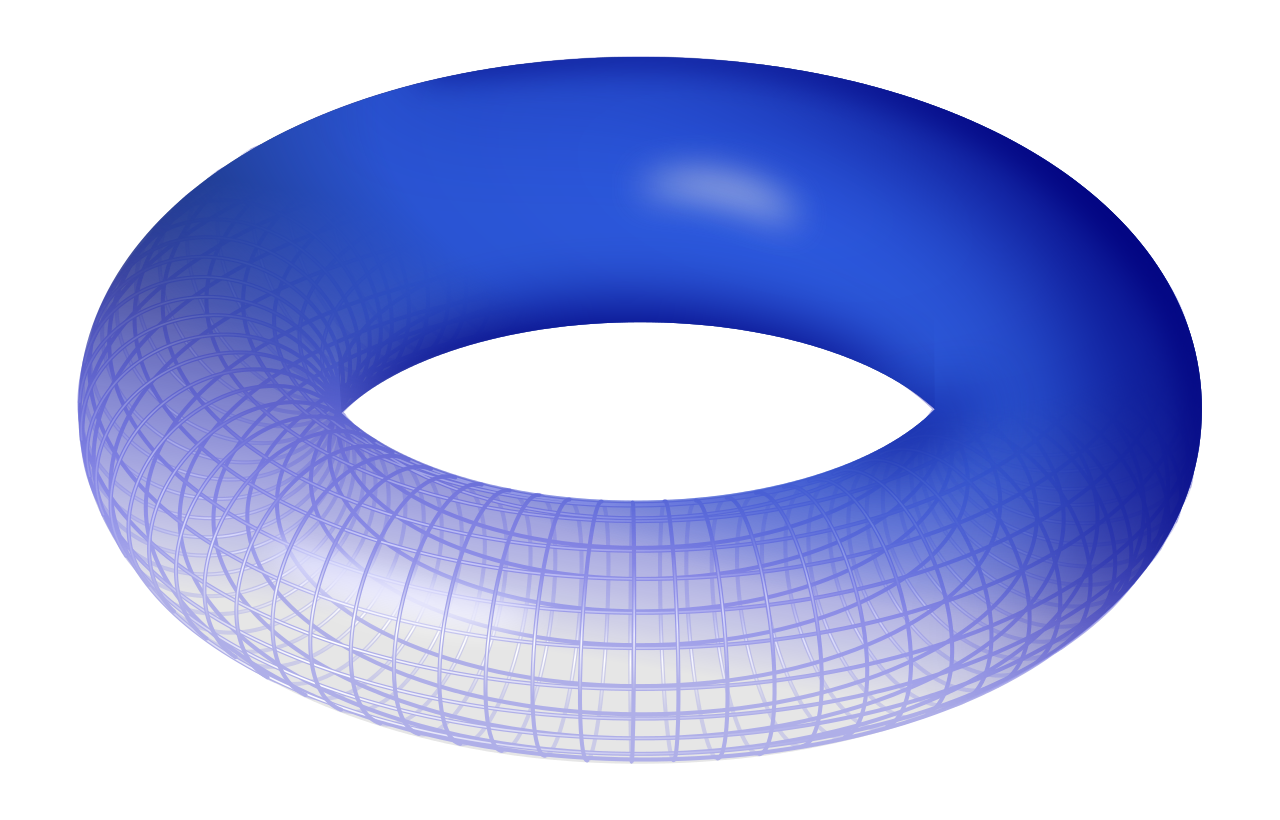
\includegraphics[width=0.5\linewidth]{images/Torus.png}
\caption{Representación clásica de un toro.}\cite{Wikipedia:Torus}
\end{figure}

La expresión paramétrica de un toro es:

\begin{equation}
\begin{tabular}{c c l}
$x$ & $=$ & $r \cos u \cos t + R \cos t$ \\
$y$ & $=$ & $r \cos u \sin t + R \sin t$ \\
$z$ & $=$ & $r \sin u$
\end{tabular}
\nonumber
\end{equation}

Si renombramos esta expresión como:

\begin{equation}\label{Uhlir03-14}
c_u = \cos u \hspace{0.5cm} c_t = \cos t \hspace{0.5cm} s_u = \sin u \hspace{0.5cm} s_t = \sin t
\end{equation}

Podemos representar la expresión paramétrica inicial en polinomios como:

\begin{equation}\label{Uhlir03-15}
\begin{tabular}{r c c}
$x - r c_u c_t - R c_t$ & $=$ & $0$ \\
$y - r c_u s_t - R s_t$ & $=$ & $0$ \\
$z - r s_u$ & $=$ & $0$
\end{tabular}
\end{equation}

La base de Gröbener reducida para el ideal $I$, generado por los polinomios (\ref{Uhlir03-14}) y (\ref{Uhlir03-15}), contiene 9 elementos. Uno solo de estos elementos no contiene variables en $c_u, s_u, c_t \text{ ó } s_t$ y tiene la forma:

$$(x^2 + y^2 + z^2 - r^2 - R^2)^2 = 4 R^2 (z^2 - r^2)$$

La cual es la expresión implícita del toro.

\subsection{Método de la resultante}

El término { \em resultante} se suele introducir si se presenta la siguiente cuestión: ¿Cuándo dos polinomios en $K[x]$ tienen un divisor común? Los métodos que usan la evaluación de la resultante se pueden usar para eliminar un subconjunto de variables del sistema inicial de ecuaciones algebraicas no lineales.
\par Un dato interesante de la resultante para polinomios en varias variables es que para $n+1$ polinomios elimina $n$ variables a la par. A diferencia del método de la base de Gröbner, este método es no secuencial. La idea básica que subyace en las resultantes multidimensionales es la conversión de un problema de eliminación no lineal en uno lineal, lo cual ayuda a aplicar métodos conocidos de Álgebra Lineal para resolver el sistema.
\par Existen distintos tipos de resultante. La definición básica involucra dos polinomios en una variable, por ejemplo la resultante de Sylvester o Bezout, y a aprtir de ahí se puede ir generalizando a dos polinomios en dos variables y después a tres polinomios en dos variables, la resultante de Dixon. Esta última puede generalizarse a $n+1$ polinomios en $n$ variables. Aquí daremos una simple pincelada para dar la idea de las resultantes ya nombradas. Podemos encontrar más información en \cite{Berchtold00}.

\subsubsection*{Resultante de Sylvester}

El principal problema es la tendencia a encontrar si dos polinomios $f, g \in K[x]$ tienen divisor común. Existenvarias maneras de encontrarlo, por ejemplo, el algoritmo de Euclides se puede usar para descomponer los polinomios en productos de factores simples. O por ejemplo, el siguiente lema.

\begin{lemma}
	Sean $f,g \in K[x]$ tales que $deg(f) = n > 0$ y $deg(g) = m > 0$ se tiene que $f$ y $g$ tienen un divisor común si y sólo si existen polinomios $A, B \in K[x]$ verificando:
	\begin{enumerate}
		\item Ambos polinomios $A$ y $B$ son no nulos.
		\item $A$ y $B$ tienen como mínimo grado $m-1$ y $n-1$ respectivamente.
		\item $Af + Bg = 0$
	\end{enumerate}
\end{lemma}

\begin{definition}
	Sean $f, g \in K[x]$ dados como $f = a_n x^n + \dotso + a_0$ y $g = b_m x^m + \dotso + b_0$ donde $a_n, b_m \neq 0$, entonces la resultante de Sylvester de $f$ y $g$ es de la forma:
	
	$$Res(f,g) = Det(Syl(f,g))$$
	
	Donde $Syl(f,g)$ denota:
	
	$$\begin{pmatrix}
	a_n & & & & & b_m & & & & \\
	a_{n-1} & a_n & & & & b_{m-1} & b_m & & & \\
	a_{n-2} & a_{n-1} & a_n & & & b_{m-2} & b_{m-1} & b_m & & \\
	\vdots & \vdots & & \ddots & \vdots & \vdots & \vdots & \vdots & \ddots & \\
	a_1 & \dotso & \dotso & \dotso & a_{n} & b_1 & \dotso & \dotso & \dotso & b_{m} \\
	a_0 & \dotso & \dotso & \dotso & a_{n-1} & b_0 & \dotso & \dotso & \dotso & b_{m-1} \\
	 & a_0 & \dotso & \dotso & a_{n-2} & & b_0 & \dotso & \dotso & b_{m-2} \\
	 & & \ddots & \vdots & \vdots & & & \ddots & \vdots & \vdots \\
	 & & & a_1 & a_0 & & & & b_1 & b_0 \\
	 & & & & a_0 & & & & & b_0
	\end{pmatrix}$$
	
	Se observa que $f$ y $g$ tienen divisores comunes si la resultante es cero.
	
\end{definition}

Ahora realizaremos un ejemplo sencillo para comparar este método con el de la base de Gröbner.
\\
\par Sean por ejemplo los polinomios:

$$f = x^2 y - 1 \hspace{2cm} g = x^2 + y^2 + xy - 4$$

Aplicando el método de la resultante de Sylvester tenemos:

$$Res(f,g) = Det \begin{pmatrix}
y & 0 & 1 & 0 \\
0 & y & y & 1 \\
-1 & 0 & y^2 - 4 & y \\
0 & -1 & 0 & y^2 - 4
\end{pmatrix} = y^6 - 8y^4 + y^3 + 16y^2 - 8y + 1$$

Para comparar podemos ver la solución obtenida mediante el método de la base de Gröbner para el ideal $I = \langle f,g \rangle$ cuya base de Gröbner reducida sería:

$$\langle x - 4y^5- y^4 + 32y^3 + 4y^2 - 64y + 16 , y^6 - 8y^4 + y^3 + 16y^2 - 8y + 1 \rangle$$

\subsubsection*{Resultante de Bezout}

Es similar a la resultante de Bezout, salvo que la definición de lamtriz de Bezout un poco más dificultosa  que la de Sylvester, pero a cambio ésta tiene dimensión $n \times n$ en lugar de la dimensión $(n+m) \times (n+m)$. En consecuencia, la evaluación del determinante de la matriz Bezout es mucho más rápido.

\subsubsection*{Resultante de Dixon}

Es una versión generalizada de la resultante y matriz de Bezout para tres polinomios en dos variables. Entonces la resultante de Dixon se generaliza para $n+1$ polinomios en $n$ variables.

\subsection{El método de Wu-Ritt}

En esta sección daremos una breve introducción a la teoría de este método. Éste se basa en la aproximación de Wu-Ritt para encontrar un conjunto característico para un sistema de ecuaciones no lineales. Dado un sistema de ecuaciones polinomiales $S = \{ f_1, \dotso, f_m \}$ se transforma en una forma triangular $S'$. Es importante notar que si el número $n$ de variables es mayor que el número de ecuaciones en un conjunto $S$ entonces el conjunto de variables se divide en dos subconjuntos: las variables independientes, que denotaremos por $\{ u_1, \dotso, u_k \}$, y ñas dependientes, que denotaremos por $\{ y_1, \dotso, y_l \}$.
\par La pseudodivisión de polinomios de varias variables es la clave en la computación de conjuntos característicos. Para realizar la pseudodivisión se da uso de la representación recursiva de los polinomios con lo cual se define una reducción polinomial.
\par Un polinomio $f_i$ se reduce respecto de otro polinomio $f_j$ si verifican una de las dos siguientes condiciones:

\begin{enumerate}
	\item La mayor variable de $f_i$ es $\prec$ la mayor variable de $f_j$.
	\item El grado de la mayor variable en $f_j$ es mayor que el grado de la mayor variable en $f_i$.
\end{enumerate} 

Si $f_i$ no es reducible respecto de $f_j$ entonces $f_i$se reduce a $r$ mediante la pseudodivisión entre $f_j$.

\begin{definition}
	Dado un conjunto finito $\Sigma$ de polinomios $u_1, \dotso, u_k, y_1, \dotso, y_l$ un conjunto característico $\Phi$ de $\Sigma$ se define de cualquiera de las siguientes maneras:
	\begin{enumerate}
		\item $\{ g_1 \}$ donde $g_1$ es un polinomio de $\{ u_1, \dotso, u_k \}$.
		\item Una cadena $\langle g_1, \dotso, g_l \rangle$ donde $g_i$ es un polinomio en $\{ u_1, \dotso, u_k, y_1, \dotso, y_i \}$ con $LC(g_i)$ tales que:
		\begin{itemize}
			\item Cualquier cero de $\Sigma$ es un cero de $\Phi$.
			\item Cualquier cero de $\Phi$ que no es cero de ninguno de los coeficientes líderes $LC(g_i)$ es un cero de $\Sigma$.
		\end{itemize}
	\end{enumerate}
\end{definition}

Podemos encontrar más información en \cite{Berchtold00}, \cite{Gallo91_2} o \cite{Gallo91_1}.